\documentclass[spanish,letterpaper,oneside]{article}

% Datos del documento
\def\documenttitle {Ecuaciones lineales y propiedades de la igualdad}
\def\documentsubtitle {Temas selectos de matemáticas I}
\def\documentsubject {Actividad 5 · Seis ecuaciones resueltas y comprobadas}
\def\documentauthor {Mtro. Martín Jonathan de la Cruz Muñoz}
\def\coursename {Temas selectos de matemáticas I}
\def\coursecode {PFM02}

% Identidad institucional
\def\universityname {Instituto de Investigación, Innovación y Estudios de Posgrado para la Educación del Estado de Nuevo León}
\def\universityfaculty {Maestría en Aprendizaje y Enseñanza de las Matemáticas}
\def\universitydepartment {Temas selectos de matemáticas I}
\def\universitydepartmentimage {img/iiiepe/marca-iiiepe.png}
\def\universitydepartmentimagecfg {height=1.75cm}
\def\universitylocation {Monterrey, Nuevo León}
\def\studentfullname {Mtro. Martín Jonathan de la Cruz Muñoz}
\def\studentid {00874}
\def\studentemail {martin.delacruz@campus.iiiepe.edu.mx}
\def\programperiod {1er tetramestre, marzo--julio de 2026}
\def\programmodality {Modalidad presencial}
\def\programshort {MAEM}

\def\authortable {
  \begin{tabular}{ll}
    \textbf{Alumno:} & \studentfullname \\
    Matrícula: & \studentid \\
    Correo institucional: & \studentemail \\
    Unidad: & \coursename \\
    Programa: & \programshort \\
    Periodo: & \programperiod \\
    & \\
    \multicolumn{2}{l}{Fecha de realización: 13 de octubre de 2026} \\
    \multicolumn{2}{l}{\universitylocation}
  \end{tabular}
}

\input{template}

\usepackage{helvet}
\renewcommand{\familydefault}{\sfdefault}
\usepackage{array}
\usepackage{longtable}
\usepackage{pdflscape}
\usepackage{tikz}
\usepackage[most]{tcolorbox}
\usetikzlibrary{arrows.meta,positioning,calc,fit,backgrounds}

\definecolor{iiiepeNavy}{HTML}{163B5C}
\definecolor{iiiepeBlue}{HTML}{1F6F9F}
\definecolor{iiiepeAqua}{HTML}{20B7A8}
\definecolor{iiiepeOrange}{HTML}{F28C28}
\definecolor{iiiepePaper}{HTML}{F6F8F7}
\definecolor{iiiepeInk}{HTML}{1E2A32}
\def\portraittitlecolor {iiiepeNavy}
\setcitestyle{authoryear,open={(},close={)}}

\newcommand{\insertcoverwatermark}{%
  \AddToShipoutPictureBG*{%
    \begin{tikzpicture}[remember picture,overlay]
      \node[opacity=.09,inner sep=0pt] at (current page.center)
      {\includegraphics[width=.58\paperwidth]{img/iiiepe/logo-puntos.png}};
    \end{tikzpicture}%
  }%
}

\newtcolorbox{reportelecturabox}[1][]{%
  enhanced,breakable,
  colback=iiiepePaper,colframe=iiiepeNavy,
  boxrule=1pt,leftrule=4pt,arc=2pt,
  left=8pt,right=8pt,top=6pt,bottom=6pt,
  before skip=6pt,after skip=10pt,
  fonttitle=\bfseries\color{white},coltitle=white,
  colbacktitle=iiiepeNavy,
  attach boxed title to top left={xshift=8pt,yshift=-2pt},
  boxed title style={colback=iiiepeNavy,colframe=iiiepeNavy,arc=1pt},
  title={Reporte de lectura},#1}

\newtcolorbox{fichalecturabox}[1][]{%
  enhanced,breakable,
  colback=iiiepeAqua!7,colframe=iiiepeAqua!70!iiiepeNavy,
  boxrule=.6pt,arc=1pt,
  left=7pt,right=7pt,top=4pt,bottom=4pt,
  fontupper=\small,before upper={\setstretch{1.0}},
  fonttitle=\bfseries\color{iiiepeNavy},coltitle=iiiepeNavy,
  colbacktitle=iiiepeAqua!7,
  title={Ficha de la lectura},#1}



\usepackage{tabularx,colortbl,pgfplots,enumitem,needspace}\pgfplotsset{compat=1.18}\definecolor{iiiepePale}{HTML}{EEF5F8}
\setlength{\parskip}{5pt}\setlength{\parindent}{0pt}
\begin{document}\insertcoverwatermark\templatePortrait\templatePagecfg\templateFinalcfg\fancyfoot{}\fancyfoot[L]{\scriptsize IIIEPE · MAEM}\fancyfoot[C]{\scriptsize\thepage}\fancyfoot[R]{\scriptsize Actividad 5}\setstretch{1.3}\raggedbottom
\section{Fases 1 y 2 · Equilibrio y ruta de solución}
Si cinco bolsas y tres canicas equilibran dos bolsas y doce canicas, $5x+3=2x+12$. Retiro dos bolsas de ambos lados, después tres canicas de ambos lados y distribuyo las nueve canicas entre tres bolsas. Cada bolsa contiene tres canicas. Lo que preserva la igualdad es aplicar la misma operación en ambos miembros; ``pasar cambiando de signo'' es una abreviatura, no una explicación.
La ruta es aplicar operaciones inversas en ambos miembros, reducir términos semejantes y comprobar. En el orden en que aparecen las opciones de la ficha: operaciones inversas (1), comprobación (3), reducción (2). En una resolución real, operaciones inversas y reducción pueden alternarse; la comprobación se realiza al final.

\begin{center}
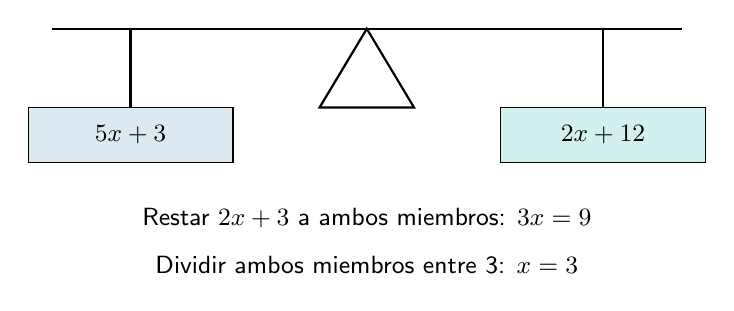
\begin{tikzpicture}[font=\small,x=1cm,y=1cm]
\draw[thick] (-4,1)--(4,1);\draw[thick] (0,1)--(-.6,0)--(.6,0)--cycle;\draw[thick] (-3,1)--(-3,0);\draw[thick] (3,1)--(3,0);
\draw[fill=iiiepeBlue!15] (-4.3,-.7) rectangle (-1.7,0);\draw[fill=iiiepeAqua!20] (1.7,-.7) rectangle (4.3,0);
\node at (-3,-.35){$5x+3$};\node at (3,-.35){$2x+12$};\node at (0,-1.4){Restar $2x+3$ a ambos miembros: $3x=9$};\node at (0,-2){Dividir ambos miembros entre 3: $x=3$};\end{tikzpicture}
\end{center}
\section{Fase 3 · Resolución completa y comprobación}
\subsection*{Nivel 1 · Enteros}


{\small\setstretch{1.1}\renewcommand{\arraystretch}{1.25}
\begin{longtable}{|>{\raggedright\arraybackslash}p{\dimexpr0.5\linewidth-2\tabcolsep-2\arrayrulewidth\relax}|>{\raggedright\arraybackslash}p{\dimexpr0.5\linewidth-2\tabcolsep-2\arrayrulewidth\relax}|}\hline
\rowcolor{iiiepePale} \textbf{Expresión} & \textbf{Procedimiento y resultado} \\\hline
\endfirsthead
\hline
\rowcolor{iiiepePale} \textbf{Expresión} & \textbf{Procedimiento y resultado} \\\hline
\endhead
$5x+3=2x+12$ & $3x=9\Rightarrow x=3$ \\\hline
$3x-7=7x+9$ & $-4x=16\Rightarrow x=-4$ \\\hline
\end{longtable}}


Comprobaciones: para $x=3$, $5(3)+3=18=2(3)+12$; para $x=-4$, $3(-4)-7=-19=7(-4)+9$.
\subsection*{Nivel 2 · Paréntesis}


{\small\setstretch{1.1}\renewcommand{\arraystretch}{1.25}
\begin{longtable}{|>{\raggedright\arraybackslash}p{\dimexpr0.5\linewidth-2\tabcolsep-2\arrayrulewidth\relax}|>{\raggedright\arraybackslash}p{\dimexpr0.5\linewidth-2\tabcolsep-2\arrayrulewidth\relax}|}\hline
\rowcolor{iiiepePale} \textbf{Expresión} & \textbf{Procedimiento y resultado} \\\hline
\endfirsthead
\hline
\rowcolor{iiiepePale} \textbf{Expresión} & \textbf{Procedimiento y resultado} \\\hline
\endhead
$2(x-4)=3(x+2)-10$ & $2x-8=3x-4\Rightarrow x=-4$ \\\hline
$4(2x+3)=2(3x-5)$ & $8x+12=6x-10\Rightarrow x=-11$ \\\hline
\end{longtable}}


Comprobaciones: $2(-4-4)=-16=3(-4+2)-10$; $4(2(-11)+3)=-76=2(3(-11)-5)$.
\subsection*{Nivel 3 · Decimales y fracciones}


{\small\setstretch{1.1}\renewcommand{\arraystretch}{1.25}
\begin{longtable}{|>{\raggedright\arraybackslash}p{\dimexpr0.5\linewidth-2\tabcolsep-2\arrayrulewidth\relax}|>{\raggedright\arraybackslash}p{\dimexpr0.5\linewidth-2\tabcolsep-2\arrayrulewidth\relax}|}\hline
\rowcolor{iiiepePale} \textbf{Expresión} & \textbf{Procedimiento y resultado} \\\hline
\endfirsthead
\hline
\rowcolor{iiiepePale} \textbf{Expresión} & \textbf{Procedimiento y resultado} \\\hline
\endhead
$0.5x+2=0.2x+3.8$ & $0.3x=1.8\Rightarrow x=6$ \\\hline
$\frac12x+3=\frac14x+5$ & $2x+12=x+20\Rightarrow x=8$ \\\hline
\end{longtable}}


Comprobaciones: $0.5(6)+2=5=0.2(6)+3.8$; $(1/2)(8)+3=7=(1/4)(8)+5$. En la última ecuación se multiplicaron ambos miembros por 4 para eliminar denominadores. La fracción se verificó en la ecuación editable del documento oficial.
\section{Resolver conservando equivalencias}
\subsection{Un ejemplo con distributiva}
La cadena $4(2x+3)=2(3x-5)$ se desarrolla como $8x+12=6x-10$. Restar $6x$ en ambos miembros produce $2x+12=-10$; restar 12 produce $2x=-22$; dividir entre 2 produce $x=-11$. Cada flecha entre ecuaciones conserva el conjunto de soluciones. La sustitución debe hacerse en la ecuación original y no únicamente en una transformación que ya pudiera contener un error.
\subsection{Un ejemplo con fracciones}
En $x/2+3=x/4+5$, multiplicar ambos miembros por 4 produce $2x+12=x+20$. Después, restar $x+12$ a ambos miembros da $x=8$. La comprobación $8/2+3=8/4+5=7$ confirma el resultado. Un error frecuente es multiplicar solo los términos fraccionarios y dejar 3 y 5 sin cambiar; una tabla de operaciones en ambos miembros ayuda a hacerlo visible.
\subsection{Un criterio para decidir el siguiente apoyo}
Si el estudiante obtiene la solución pero no justifica una transformación, solicitaría nombrar la operación aplicada a ambos miembros. Si la dificultad está en signos, trabajaría primero $-3+7$ con recta numérica. Si la dificultad está en la distributiva, contrastaría $2(x+3)$ con $2x+3$ mediante un valor. Este diagnóstico distingue obstáculos y evita repetir toda la explicación a quien necesita un apoyo específico.
\section{Secuencia de aplicación y evaluación}
Resolver ecuaciones conservando el conjunto de soluciones. La duración propuesta es de 80 minutos, ajustable al diagnóstico y a los recursos. Esta planeación sigue la progresión de los recursos institucionales (IIIEPE, 2026); los tiempos y apoyos son decisiones de codiseño, no datos de una aplicación ya realizada.

{\small\setstretch{1.1}\renewcommand{\arraystretch}{1.25}
\begin{longtable}{|>{\raggedright\arraybackslash}p{\dimexpr0.23\linewidth-2\tabcolsep-2\arrayrulewidth\relax}|>{\raggedright\arraybackslash}p{\dimexpr0.49\linewidth-2\tabcolsep-2\arrayrulewidth\relax}|>{\raggedright\arraybackslash}p{\dimexpr0.28\linewidth-2\tabcolsep-2\arrayrulewidth\relax}|}\hline
\rowcolor{iiiepePale} \textbf{Fase y tiempo} & \textbf{Actividad y mediación} & \textbf{Evidencia} \\\hline
\endfirsthead
\hline
\rowcolor{iiiepePale} \textbf{Fase y tiempo} & \textbf{Actividad y mediación} & \textbf{Evidencia} \\\hline
\endhead
1. Reto y saberes (10 min) & Representar el equilibrio de bolsas y canicas. & Predicción individual y pregunta. \\\hline
2. Plan de indagación (15 min) & Planear operaciones equivalentes en ambos miembros. & Plan explicado y criterios. \\\hline
3. Construcción y análisis (25 min) & Resolver enteros, distributiva y fracciones con apoyos graduados. & Registro o procedimiento trazable. \\\hline
4. Comunicación y aplicación (18 min) & Comprobar en la ecuación original y explicar una transformación. & Argumento con comprobación. \\\hline
5. Metacognición (12 min) & Corregir un paso y transferir a dos costos de mantenimiento. & Versión revisada y justificación. \\\hline
\end{longtable}}
\subsection{Criterios observables y retroalimentación}

{\small\setstretch{1.1}\renewcommand{\arraystretch}{1.25}
\begin{longtable}{|>{\raggedright\arraybackslash}p{\dimexpr0.22\linewidth-2\tabcolsep-2\arrayrulewidth\relax}|>{\raggedright\arraybackslash}p{\dimexpr0.4\linewidth-2\tabcolsep-2\arrayrulewidth\relax}|>{\raggedright\arraybackslash}p{\dimexpr0.38\linewidth-2\tabcolsep-2\arrayrulewidth\relax}|}\hline
\rowcolor{iiiepePale} \textbf{Criterio} & \textbf{Evidencia de logro} & \textbf{Acción si necesita apoyo} \\\hline
\endfirsthead
\hline
\rowcolor{iiiepePale} \textbf{Criterio} & \textbf{Evidencia de logro} & \textbf{Acción si necesita apoyo} \\\hline
\endhead
Equivalencia & Explica equivalencia con un caso de la actividad. & Pedir una representación concreta y contrastar dos casos. \\\hline
Distributiva y signos & Conserva distributiva y signos en el desarrollo y justifica sus pasos. & Modelar un paso, retirar gradualmente la ayuda y solicitar otro caso. \\\hline
Despeje & Utiliza despeje para contrastar una respuesta o representación. & Comparar la evidencia inicial y la corregida con una pregunta específica. \\\hline
Comprobación original & Relaciona comprobación original con la conclusión y un límite del problema. & Solicitar una comprobación independiente y un caso de transferencia. \\\hline
\end{longtable}}
El instrumento es una propuesta docente. Cada criterio se registra como logrado con autonomía, logrado con apoyo o aún no demostrado; no se asigna una calificación observada sin aplicar la actividad. En la coevaluación, un compañero verifica un criterio y formula una pregunta; en la autoevaluación, el estudiante explica una corrección; el docente contrasta ambas evidencias y decide el siguiente apoyo.\subsection{Participación y apoyos}
La inclusión se concreta en alternativas de representación y de acceso; el pensamiento crítico, en justificar y contrastar. Los roles de cálculo, registro y explicación se rotan para que todos produzcan una evidencia individual. Quien necesita apoyo dispone de un ejemplo parcial y preguntas graduadas; quien ya domina el procedimiento analiza un contraejemplo o cambia una condición. Estas acciones deben observarse durante la aplicación para valorar su funcionamiento.

\section{Fases 4 y 5 · Presentación y metacognición}
El procedimiento exige revisar la propiedad distributiva y los signos antes de simplificar; una comprobación independiente permite detectar errores que un resultado aislado oculta. Un problema de extensión para el hogar sería comparar dos servicios de mantenimiento: $C_A=250+80h$ y $C_B=100+110h$. Igualando, $150=30h$, de modo que coinciden en $h=5$ horas y $C=650$ pesos. Por debajo de 5 horas conviene B; por encima, A, si el servicio es equivalente.
No marcaría automáticamente la autoevaluación de participación ni declararía una entrega en tiempo: son evidencias personales y administrativas que requieren validación. Matemáticamente sí quedan demostradas las seis soluciones y sus comprobaciones.
\section{Reflexión sobre el diseño didáctico}
Para un grupo con rezago en operaciones y signos conservaría el reto de la balanza, pero incorporaría una etapa de fichas positivas y negativas, un ejemplo resuelto y ejercicios con un solo cambio por vez. La progresión sería $3x=9$, $3x+2=11$, $5x+3=2x+12$ y finalmente distributiva. Ofrecería una recta numérica y permitiría explicar oralmente antes de escribir. El apoyo cambia, pero el objetivo de comprender equivalencia permanece.
La entrega digital debe cerrar un ciclo formativo: una devolución breve identifica un paso logrado, un error concreto y una acción de mejora; el estudiante publica la corrección y una comprobación. En una sesión posterior, un problema equivalente sin ayuda permite revisar comprensión. En CONALEP, CECyTE y las ingenierías, vincularía este ciclo con ajustes y diagnóstico técnico, incorporando atención a las condiciones de acceso y al tiempo disponible de los estudiantes.

\needspace{5\baselineskip}\section*{Referencias}
{\setstretch{1.15}\setlength{\parskip}{6pt}
\par\hangindent=1.27cm\hangafter=1  Academia Estatal de Matemáticas. (2023). \textit{Practicando saberes en Matemáticas: Cuaderno de trabajo. Primer grado. Secundaria}. Secretaría de Educación de Nuevo León.
\par\hangindent=1.27cm\hangafter=1  IIIEPE. (2026). \textit{Recurso sesión 5: Ecuaciones lineales y cuadráticas}. EVA posgrado.
\par\hangindent=1.27cm\hangafter=1  Secretaría de Educación Pública. (2024). \textit{Programa de estudio para la educación secundaria: Programa sintético de la Fase 6}. SEP.
}

\end{document}
